PID kontrolör
\begin{equation}
    F(s)=k_p+\frac{k_i}{s}+k_d s
\end{equation}
olmak üzere kapalı çevrim transfer fonksiyonu 
\begin{equation}
\begin{split}
    T(s)&=\frac{F(s)G(s)}{1+F(s)G(s)}\\
    &=\frac{\frac{k_ds^2+k_ps+k_i}{s}\frac{1}{s^2+s+1}}{1+\frac{k_ds^2+k_ps+k_i}{s}\frac{1}{s^2+s+1}}\\
    &=\frac{k_ds^2+k_ps+k_i}{s^3+(k_d+1)s^2+(k_p+1)s+k_i}
\end{split}
\end{equation}
olarak elde edilmektedir. 3. dereceden bir kapalı çevrim karakteristik polinom elde edilmesi sebebiyle 
isterleri sağlayacak polinom
\begin{equation}
\begin{split}
    p(s)&=(s^2+2\zeta\omega_n s+\omega_n^2)(s+p)\\
    &=(s^2+8s+45.7844)(s+p)\\
    &=s(s^2+8s+45.7844)+p(s^2+8s+45.7844)\\
    &=s^3+8s^2+45.7844s+ps^2+8ps+45.7844p\\
    &=s^3+(p+8)s^2+(8p+45.7844)s+45.7844p
\end{split}
\end{equation}
kullanılmalıdır.
Tasarım için problem
\begin{equation}
\begin{split}
    k_d+1&=p+8\\
    k_p+1&=8p+45.7844\\
    k_i&=45.7844p
\end{split}
\end{equation}
olarak tanımlanmaktadır. 4 bilinmeyen 3 denklem için sonsuz farklı çözüm mevcuttur. Parametrik çözüm 
\begin{equation}
\begin{split}
    k_d&=p+7\\
    k_p&=8p+44.7844\\
    k_i&=45.7844p
\end{split}
\end{equation}
olarak elde edilir ve $p$ parametresi pozitif seçilebilir. Kapalı çevrim transfer fonksiyonu 
\begin{equation}
\begin{split}
    T(s)&=\frac{(p+7)s^2+(8p+44.7844)s+45.7844p}{s^3+(p+8)s^2+(8p+45.7844)s+45.7844p}
\end{split}
\end{equation}
olarak elde edilmektedir. İsterlerin sağlanması için seçilen kapalı çevrim transfer fonksiyonu
\begin{equation}
\begin{split}
    T(s)&=\frac{45.7844p}{s^3+(p+8)s^2+(8p+45.7844)s+45.7844p}
\end{split}
\end{equation}
ve $p\geq 5\zeta\omega_n$ olmalıdır. Fakat, pay ifadesi iki adet sıfır içermektedir ve bu sıfırların da 5 kat uzakta olması gerekmektedir. Hem 3. kutbu hem de sıfırları en uzağa yerleştirecek $p$ değeri tarama yöntemi ile
\begin{equation}
\begin{split}
    p&=19.9\\
    k_p&=203.984\\
    k_d&=26.9\\
    k_i&=911.11
\end{split}
\end{equation}
ve kapalı çevrim transfer fonksiyonu
\begin{equation}
    T(s)=\frac{26.9 s^2 + 204 s + 911.1}{s^3 + 27.9 s^2 + 205 s + 911.1}
\end{equation}
olarak hesaplanmıştır. Basamak yanıtı Şekil~\ref{fig:pid_kontrol} ile gösterilmektedir.
\begin{figure}[!htb]
    \centering
    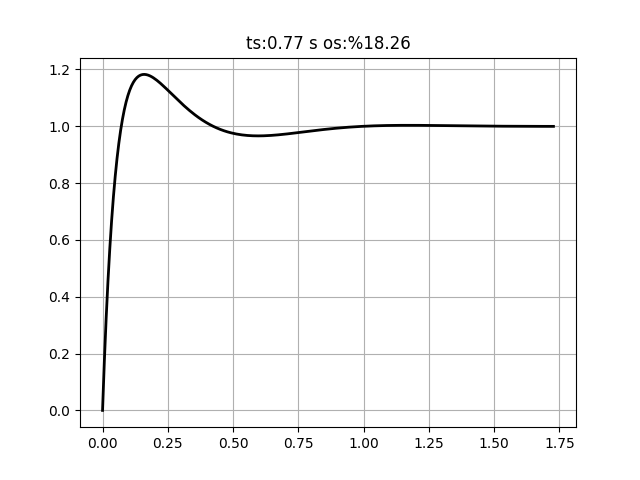
\includegraphics[width=0.75\textwidth]{pid_kontrol}
    \caption{PID kontrolör}
    \label{fig:pid_kontrol}
\end{figure}